\section{Photovoice, multiletramentos e pedagogia psicodramática: uma possibilidade 
	de diálogo virtual na pandemia}\label{sec-Photovoice,multiletramentos}
	
Para a prática de ensino discutida neste trabalho, combinamos a técnica \textit{Photovoice} \cite{wang_photovoice:_1997} com os pressupostos didático-metodológicos da Pedagogia Psicodramática \cite{romana_pedagogia_2019} aliadas ao trabalho com linguagens na perspectiva dos multiletramentos. Para efeito de análise dos dados, utilizamos os quatro processos de conhecimento propostos por \textcite{cope_letramentos_2020}: experienciar o novo; conceitualizar com teoria; aplicar criativamente; e analisar criticamente.

A Pedagogia dos Multiletramentos, conforme \textcite{cope_letramentos_2020}, tem apontado para a multiplicidade de linguagens e meios (mídias) pelos quais se dão as interações humanas na contemporaneidade, o que requer uma educação, especialmente no contexto do ensino de línguas, conectada com essa realidade. Trata-se de uma abordagem que propõe uma maneira de pensar o processo de ensino e aprendizagem mais conectada com a realidade sociocultural dos aprendizes, priorizando, assim, práticas mais significativas.

A Pedagogia Psicodramática, criada pela pedagoga argentina Maria Alicia Romaña, fundamentada em Jacob Levy Moreno, Paulo Freire e Vigotski, propõe o uso de recursos variados no processo de ensino e aprendizagem, como o trabalho de grupo, o jogo, o teatro, a expressão corporal, visando desenvolver, por meio de atividades lúdicas, a espontaneidade e a criatividade, o que possibilita que os alunos possam refletir criticamente sobre si mesmos, as relações com o(s) outros(s) e com o mundo, favorecendo a construção coletiva do conhecimento.

Para \textcite{romana_pedagogia_2019}, as práticas pedagógicas se constituem a partir de temas norteadores (temas protagônicos), que emergem das vivências/atividades em grupo, conforme a configuração e as necessidades dos aprendizes no aqui e agora. Sendo assim, as atividades desenvolvidas no projeto de ensino citado neste artigo foram todas planejadas e implementadas conforme as etapas propostas pela autora, a saber: 1) \textit{Aquecimento Inespecífico (AI)}; 2)\textit{ Aquecimento Específico (AE)}; 3) \textit{Dramatização (DR)}; e 4) \textit{Compartilhamento (COMP)}.

Dessa forma, os meses de abril e maio de 2021 foram reservados ao \textit{aquecimento inespecífico}, momento em que tivemos organização dos participantes em equipes, segundo o critério “maior afinidade com a área do conhecimento”. Durante reunião da equipe de professores e a apresentação da proposta do projeto em encontro virtual síncrono aos participantes, foram formadas sete equipes. Na sequência (maio), tivemos dois encontros síncronos por equipe, cuja temática norteadora foi “Eu, tu, nós: valorização do eu, respeito ao outro”, momento em que os professores trabalharam com músicas, vídeos, jogos, contos, fábulas, vivências em grupo, \textit{gifs}, fotografias para despertar a atenção dos participantes acerca das questões inerentes ao cuidado do eu e das relações eu-outro. As ações realizadas no projeto tinham como propósito criar espaços de fala, de escuta atenta, de solidariedade e de troca entre os estudantes e professores. Temos uma produção realizada, nessa etapa, pelos estudantes da equipe da área de enfermagem, via Padlet (\Cref{fig-01}):

\begin{figure}[htbp]
\centering
\begin{minipage}{.9\textwidth}
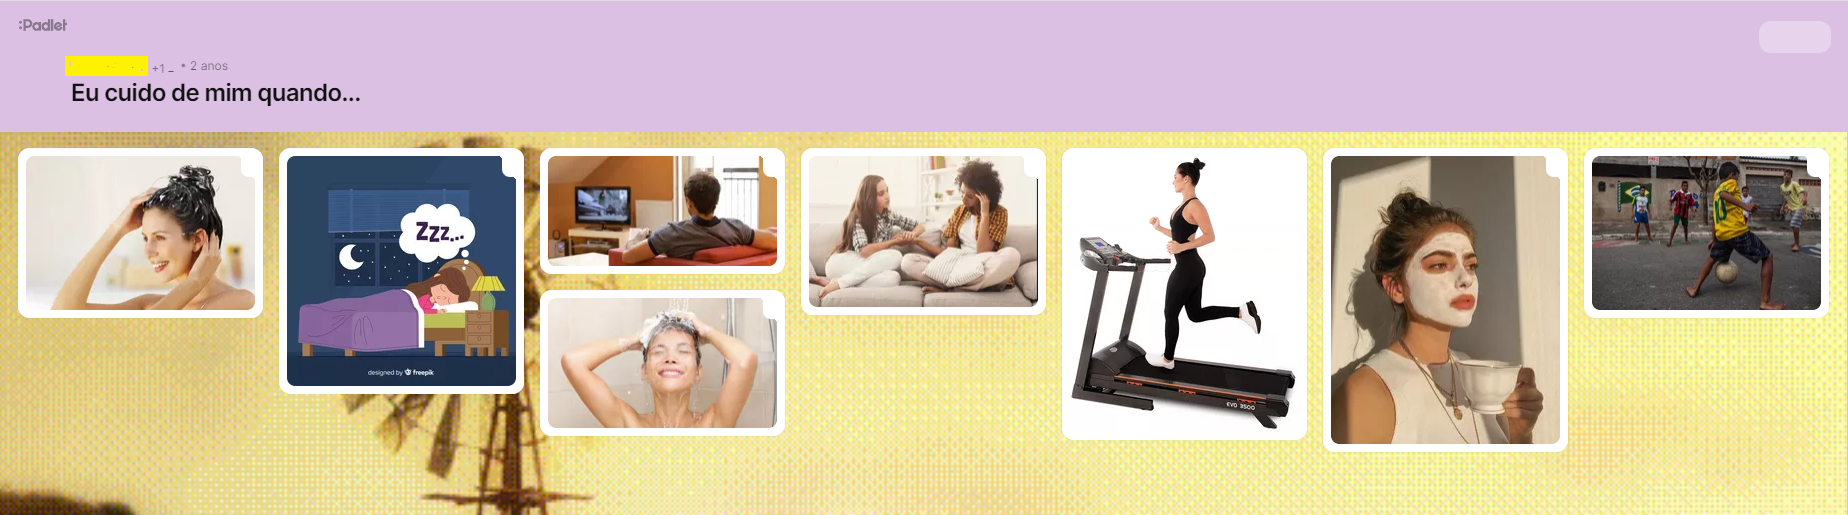
\includegraphics[width=\textwidth]{figure01.png}
\caption{Padlet criado pela equipe de enfermagem.}\label{fig-01}
\source{Arquivo pessoal.}
\end{minipage}
\end{figure}
 
Nesse caso, a professora da área pediu para que os alunos colocassem uma imagem no Padlet, criado inicialmente por ela, tendo por base a consigna “Eu cuido de mim quando…”. O intuito era trazer à discussão o repertório dos alunos acerca do cuidado do eu e do outro. A partir das imagens compartilhadas, a mediadora fez algumas perguntas aos participantes como: {\textquotedbl}\textit{Alguém do grupo pratica isso?”, “Como essas práticas relacionam-se com outras pessoas/meio ambiente?”, “Quando praticamos o que vocês trouxeram, podemos impactar o outro e o meio ambiente de alguma forma?”.}

A partir dessa etapa, os participantes “experienciaram o conhecido”, suas próprias visões do que entendiam sobre cuidado de si e do outro, ao mesmo tempo em que “experienciaram o novo”, à medida que iam visualizando/escutando o entendimento dos colegas e as considerações da professora da área de enfermagem acerca do conceito de saúde e autocuidado. Além disso, alguns deles também não conheciam a ferramenta Padlet. Na ocasião, puderam também “analisar criticamente”, quando discutiram sobre a importância do sono noturno e da prática de atividades físicas para a saúde e bem-estar, dos prejuízos causados por uma rotina de muito trabalho e de bombardeio de informações, que configuram nossa sociedade neoliberalista, do excesso de uso de telas e dos lucros que grandes empresas obtêm a partir desse consumo desenfreado da internet; além disso, discutiram o quanto esse padrão de sociedade e as nossas escolhas e estilos de vida podem equilibrar/desequilibrar o meio ambiente e o quanto isso pode contribuir ou não para o bem-estar, saúde humana e justiça social.  

No \textit{aquecimento específico}, as ações propostas buscaram o envolvimento direto dos participantes para a abordagem do tema central (neste caso, o cuidado tridimensional), preparando-os para assumir o protagonismo dentro do processo. Durante junho e julho, alunos e professores, norteados pela temática “Unidos venceremos”, desenvolveram atividades voltadas para o levantamento de questões socioambientais que impactavam/afetavam, conforme o olhar dos participantes, o “eu”, o “outro” e o “meio ambiente”. Para isso, foram realizadas atividades síncronas e assíncronas, como uma oficina virtual em que trabalhamos a análise coletiva de fotografias, o direito de imagem, o direito autoral, dicas de registro de fotografias, o aplicativo Comica e as características da técnica \textit{photovoice}, além de dois encontros síncronos por equipe, conforme a temática norteadora do mês.

Dessa forma, durante o AE, os participantes, a partir do que já conheciam e do que aprenderam no AI acerca do cuidado tridimensional, puderam “experienciar o novo” levantando as seguintes questões socioambientais: a) respeito e empatia (língua portuguesa); b) ética e ecologia (filosofia); c) consequências do desmatamento para indígenas, quilombolas e pescadores (sociologia); d) voçoroca\footnote{ Formação de grandes buracos de erosão causados pela chuva e intempéries, em solos onde a vegetação é escassa e não mais protege o solo, que fica cascalhento e suscetível de carregamento por enxurradas \cite{gomes_formacao_2021}.} (geografia); e) mapeamento socioambiental (biologia); f) saúde mental (enfermagem); g) o “eu” como agente potencial para a mudança no mundo (psicologia).

A partir do levantamento dos sete temas protagônicos citados acima, a equipe de professores aplicou um questionário para levantar a temática de maior interesse entre todos os participantes, sendo que a maioria deles optou pelo tema “saúde mental” (\Cref{fig-02}):

\begin{figure}[htbp]
\centering
\begin{minipage}{.9\textwidth}
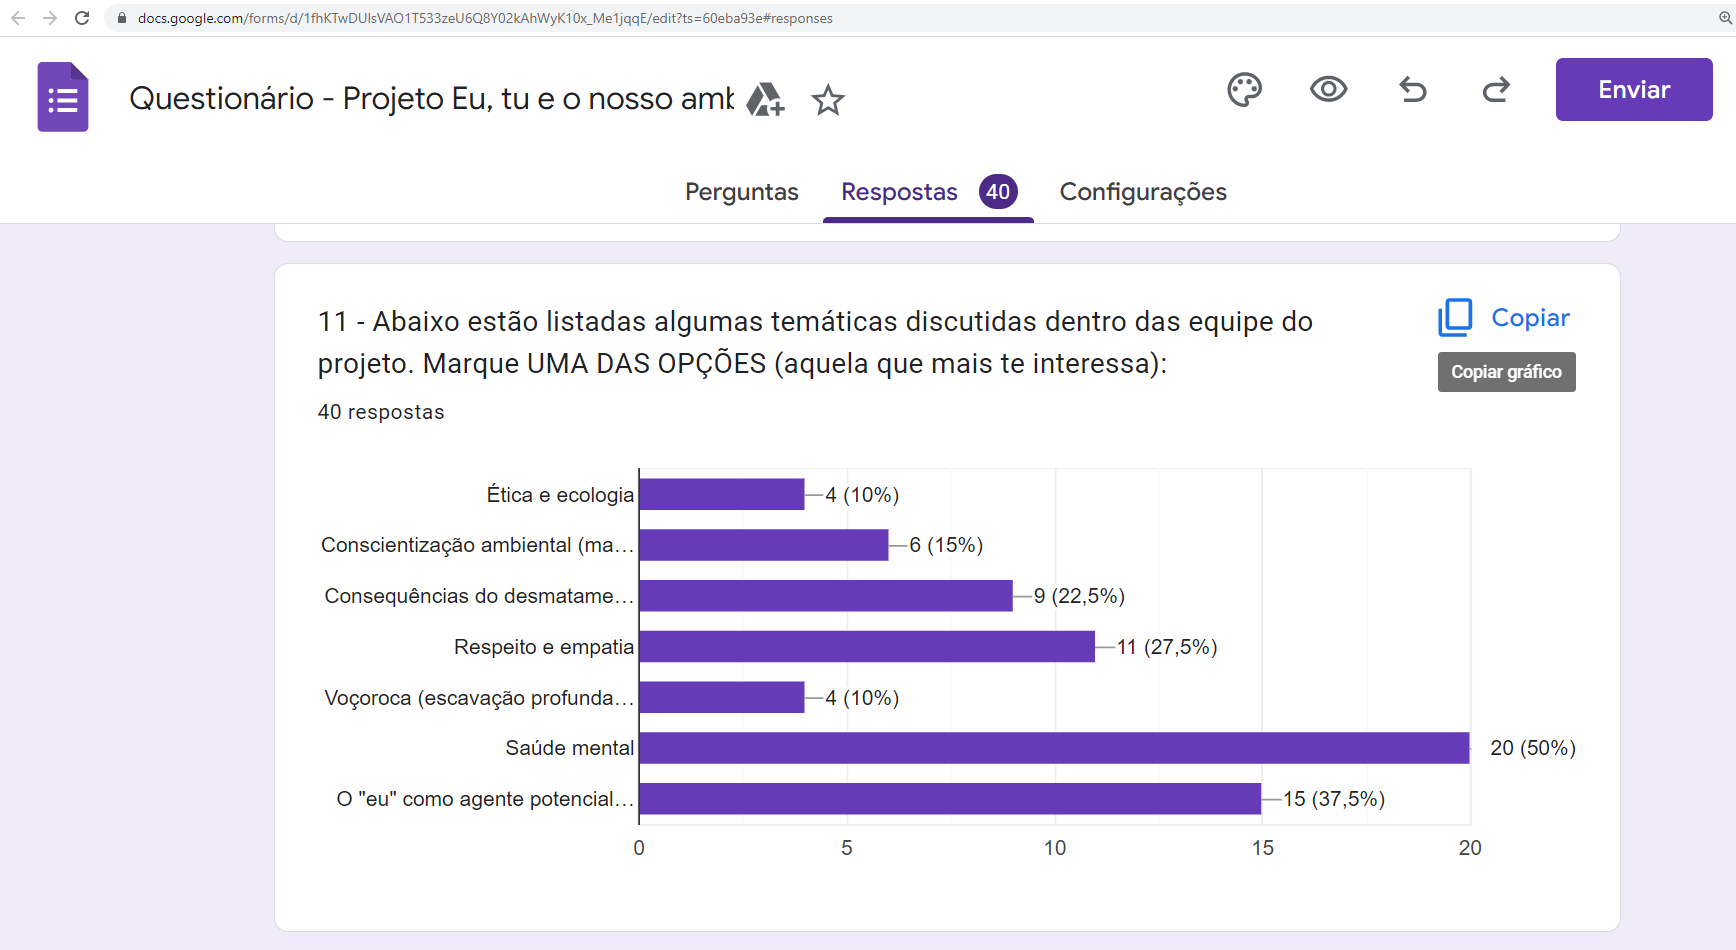
\includegraphics[width=\textwidth]{figure02.png}
\caption{Temática protagônica escolhida pelos participantes do projeto.}\label{fig-02}
\source{Arquivo pessoal.}
\end{minipage}
\end{figure}
  
Após consulta aos participantes, conforme a \Cref{fig-02}, nós professores organizamos e realizamos atividades diversificadas que atendessem, cada área à sua maneira, os temas emergidos das equipes, em especial focamos no autocuidado, nas relações respeitosas e empáticas com o(s) outro(s) e com o meio ambiente para a promoção da saúde mental e bem-estar da coletividade.

Fechamos o primeiro semestre (2021/1) realizando um encontro geral com a presença de todas as equipes e professores para compartilhamento e trocas das experiências de aprendizagem. Os participantes foram desafiados a encontrar uma forma criativa para socializar os aprendizados entre as equipes. “Aplicando criativamente” os conhecimentos adquiridos, a equipe de Língua Portuguesa lançou mão da teatralização para apresentar situações empáticas e respeitosas nas relações interpessoais como o uso de máscara e a vacinação na pandemia, abordando e refletindo os prejuízos coletivos quando não temos \textit{respeito} e \textit{empatia} nas relações sociais, em especial, no contexto pandêmico (negativismo, recusa de uso de máscaras e álcool para higienização das mãos e ambientes, queima de lixo no quintal de casa e o impacto disso para a coletividade).

Nesse contexto, a equipe de filosofia, também “aplicando criativamente”, explorou a linguagem imagética e produziu a “árvore filosofal” (\Cref{fig-03}), cheia de frutos, para compartilhar conceitos relacionados ao cuidado tridimensional. Desse modo, conforme argumentou a equipe, temos o seguinte: fruto 1 representa o planeta terra e tudo o que nele existe, o qual necessita de frutos como \textit{união} (2), \textit{colaboração} (3, 7 e 8), \textit{sabedoria} (4)\footnote{ Imagem de uma águia que representa a sabedoria, conceito discutido a partir da fábula “A águia que quase virou galinha”, de Rubem Alves, nas aulas com a equipe de filosofia.}, \textit{respeito} (5), \textit{hospitalidade e convivência} (6), \textit{acolhimento} e \textit{solidariedade} (9) e \textit{cuidado} (11 e 12). Por outro lado, o grupo “analisando criticamente” trouxe o fruto 13 simbolizando algo ruim, o não cuidado com o planeta, destacando o consumo desenfreado que resulta em grande quantidade de lixo. Os alunos encerraram o compartilhamento com a seguinte frase: “Para a ganância, toda a natureza é insuficiente” (Sêneca).  


\begin{figure}[htbp]
\centering
\begin{minipage}{.9\textwidth}
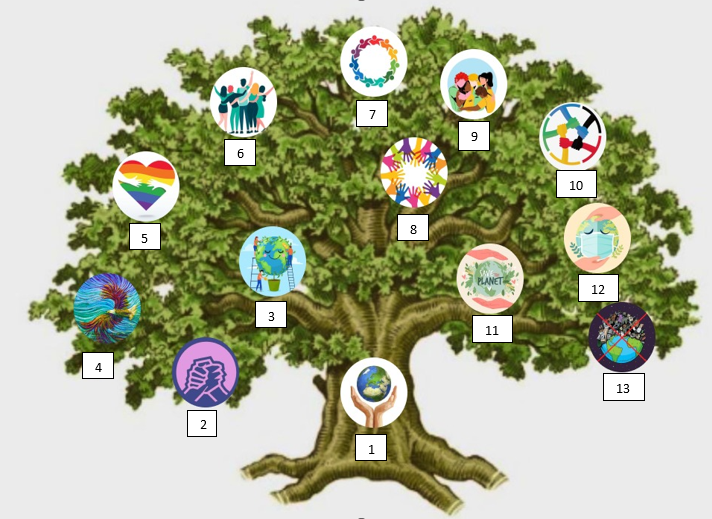
\includegraphics[width=\textwidth]{figure03.png}
\caption{A árvore filosofal produzida pela equipe de Filosofia.}\label{fig-03}
\source{Arquivo pessoal.}
\end{minipage}
\end{figure}
 

Na terceira etapa, \textit{dramatização}, momento “mão na massa”, realizada entre setembro e outubro, os estudantes, interagindo uns com outros, produziram fotografias registrando situações cotidianas que afetavam a tríade eu-outro-meio ambiente, norteados pela pergunta: \textit{Quais problemáticas socioambientais presentes em vossas realidades afetam o eu, o outro e o meio ambiente?} Nesta etapa, foi criado um mural fotográfico (\Cref{fig-04}), por meio da ferramenta Padlet, onde os estudantes iam armazenando as fotografias registradas. O mural era aberto a todos os participantes, que foram incentivados à utilização de fotografias uns dos outros, respeitando o direito autoral e dando o devido crédito ao(s) autor(es).

\begin{figure}[htbp]
\centering
\begin{minipage}{.9\textwidth}
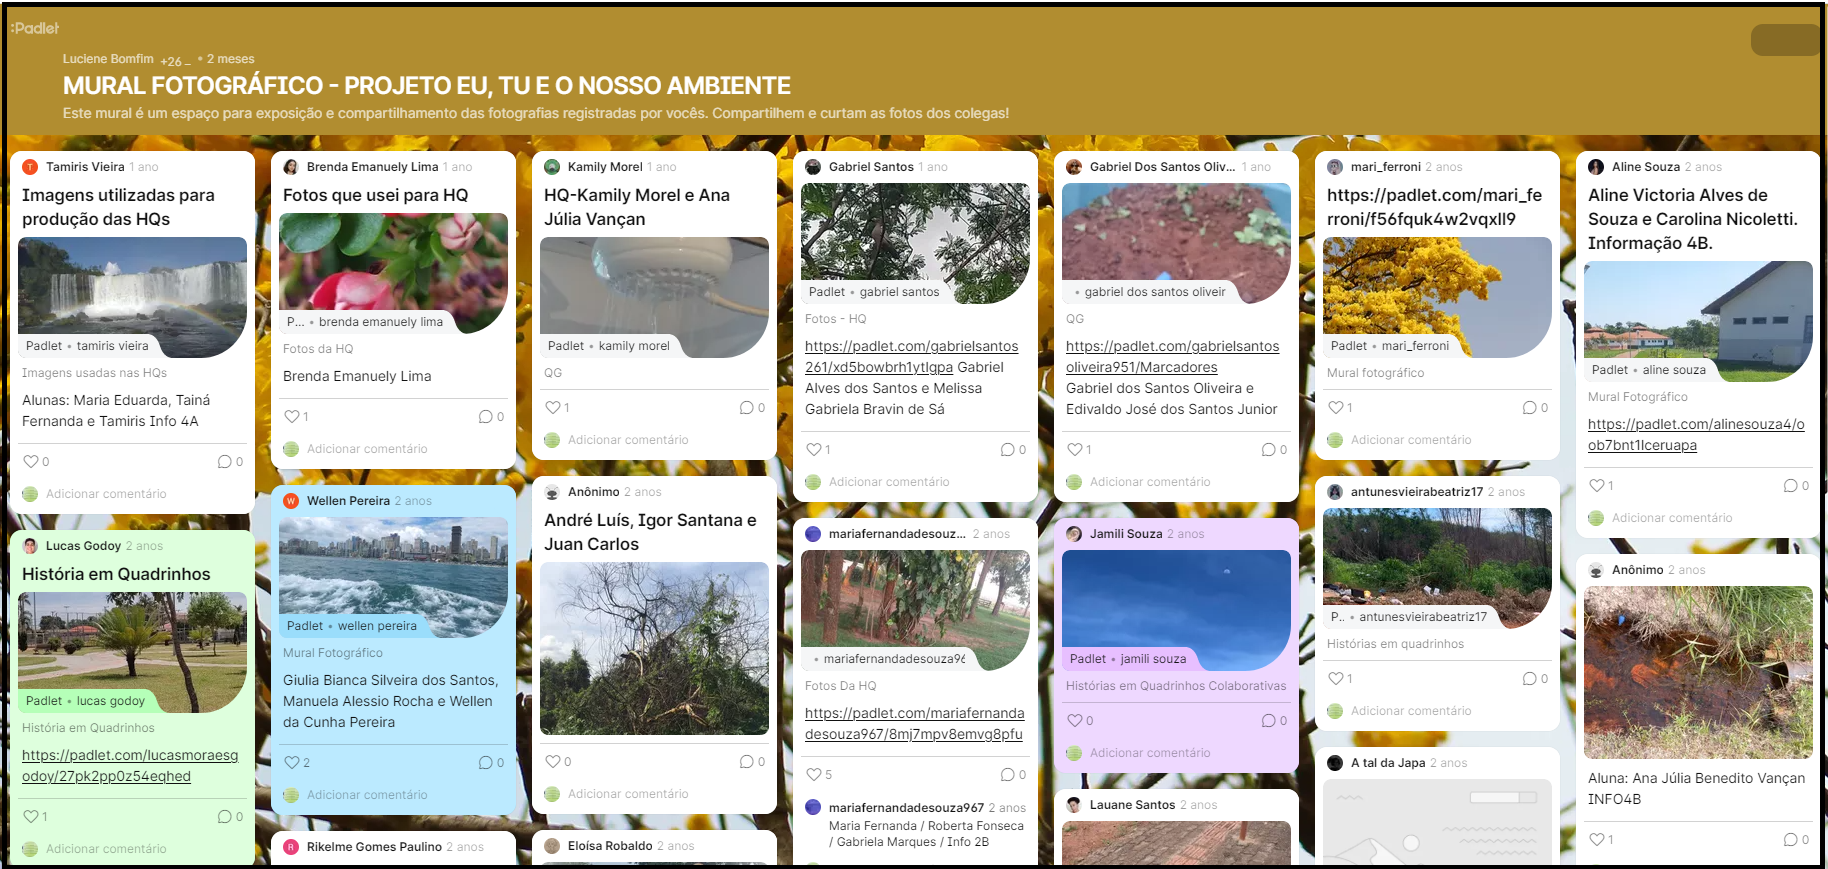
\includegraphics[width=\textwidth]{figure04.png}
\caption{Mural fotográfico do Projeto Eu, tu e o nosso ambiente.}\label{fig-04}
\source{Arquivo pessoal.}
\end{minipage}
\end{figure}
  
Para os registros fotográficos foi utilizada a técnica \textit{photovoice}, criada por \textcite{wang_photovoice:_1997}, a qual utiliza a fotografia para que as pessoas possam identificar/levantar questões importantes em suas comunidades, com o intuito de refletir e entender as suas realidades, buscando transformá-las (o que vai ao encontro da {\textquotedbl}prática transformada{\textquotedbl} prevista na teoria dos multiletramentos. As fotografias produzidas pelos participantes foram utilizadas para a construção de narrativas pessoais e em grupo/colaborativas, a partir da mixagem de linguagens verbais (escrita ou oral) e imagética. Os registros fotográficos evidenciaram dimensões tanto individual quanto colaborativa e social; além disso, serviram de base para as produções textuais multissemióticas (Histórias em Quadrinhos – HQs – e vídeos).

“Aplicando criativamente” o que aprenderam nas atividades do projeto, os participantes produziram vinte e duas Histórias em Quadrinhos, gênero textual bastante comum ao universo infanto-juvenil, as quais “por meio de seus enredos, ajudam os leitores [e autores] a ajustar suas personalidades à época e ao mundo” \cite[p. 34]{carvalho_educacao_2007}. Além disso, é um gênero que possibilita a exploração de diversos assuntos/temas; sendo assim, “analisando criticamente” os participantes exploraram as seguintes temáticas nas HQs: 

\begin{enumerate*}[label=\arabic*)]
	\item Reciclagem;
	\item preservação ambiental;
	\item desperdício de água;
	\item confiança nas relações interpessoais;
	\item importância da chuva para a vida;
	\item exclusão social;
	\item descarte inadequado de lixo;
	\item ameaça à biodiversidade;
	\item solidão;
	\item animais em situação de rua;
	\item falta de acessibilidade;
	\item queimadas;
	\item voçorocas.
\end{enumerate*}

Apropriando-se de múltiplas linguagens e recursos digitais, e a partir do olhar atento ao cotidiano motivado pelos professores das áreas envolvidas no projeto, os alunos produziram sentidos por meio de textos autorais e criativos. Para \textcite[p. 307]{santos_letramento_2011}, a produção das HQs não pressupõe apenas “juntar palavras e imagens, antes, relacioná-las” no processo de produção de sentido.

A etapa final do projeto foi reservada ao \textit{compartilhamento }(novembro e dezembro)\textit{, }momento em que os participantes, “aplicando criativamente”, socializaram o conhecimento em eventos institucionais como a Semana de Ciência e Tecnologia (roda de conversa entre professores e alunos) e o Festival de Arte e Cultura (apresentação de vídeos) do IFMS. Além disso, ainda “analisando criticamente”, fizemos um encontro síncrono \textit{on-line} com músicas selecionadas pelos participantes cujas letras relacionavam-se com o cuidado tridimensional; “teia” de agradecimentos afetuosa entre os participantes; jogos em grupos que abordaram assuntos relacionados ao projeto, além da apresentação de uma paródia da música \textit{Será}\footnote{ Para acesso à paródia, acesse: \url{https://drive.google.com/file/d/166ss42qra_vChO5tjLIKRmCSbi_G13b6/view?usp=sharing}.}, do grupo Legião Urbana, em que a equipe da geografia abordou e analisou criticamente o problema das voçorocas que afetam a cidade de Nova Andradina e a região do vale do Ivinhema, no Mato Grosso do Sul.

É importante ressaltar que os quatro processos do conhecimento não são lineares. Cada prática pedagógica tem um propósito e a depender disso é que os envolvidos no processo vão explorando-os de acordo com os objetivos de aprendizagem e os resultados pretendidos, conforme notamos em nosso projeto e buscamos ilustrar aqui.
